\documentclass{article}

\usepackage[printqrbox=false,printhint=true,printanswer=true,printmarkingguide=false]{unswalgos}

\usepackage{tikz}
\usetikzlibrary{patterns}
\usetikzlibrary{shapes,fit}
\usepackage{tkz-fct}
\usepackage{wrapfig}
\usepackage{subfig}

\usepackage{mathtools}
\usepackage{amssymb}
\usepackage{booktabs,multicol,multirow}
\usepackage{wasysym}
\usepackage{tcolorbox}

\DeclareMathOperator*{\argmax}{arg\,max}
\DeclareMathOperator*{\argmin}{arg\,min}
\DeclareMathOperator{\NAND}{NAND}
\DeclareMathOperator{\AND}{AND}
\DeclareMathOperator{\OR}{OR}
\DeclareMathOperator{\NOT}{NOT}

\usepackage{xspace}

\fancyfoot[L]{\leftmark}
\fancyfoot[R]{\rightmark}

% This enables new paragraphs without indentation
\usepackage[parfill]{parskip}

\newcommand{\sem}{23T1}
\newcommand{\semester}{Term 1, 2023}
\SubjectNo{COMP3121/9101}
\newcommand{\taskname}{Assignment 1, Question 3}
\Institution{Caleb Watts, z5360175} % Replace this with your name and zID


\begin{document}

\setcounter{question}{2}

\begin{Question}
A \emph{traversal} of a binary tree is an order in which one can visit all the nodes.
\begin{itemize}
    \item In-order traversal first recurses on the left subtree, then visits the root node, and recurses on the right subtree.
    \item Pre-order traversal first visits the root node, then recurses on the left subtree, and finally recurses on the right subtree.
    \item Post-order traversal first recurses on the left subtree, then recurses on the right subtree, and finally visits the root node.
\end{itemize} 

For example, the tree given below has:
\begin{itemize}
    \item in-order traversal of $[1, 8, 9, 5, 6, 3, 2]$,
    \item pre-order traversal of $[5, 8, 1, 9, 3, 6, 2]$, and
    \item post-order traversal of $[1, 9, 8, 6, 2, 3, 5]$.
\end{itemize}

\begin{center}
    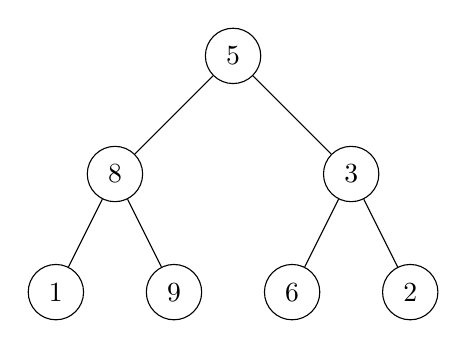
\begin{tikzpicture}[-,>=stealth',level/.style={sibling distance = 3cm/#1,
        level distance = 1.5cm}, transform shape]
    \node [circle,draw,minimum size=2em] {5}
    child{ node [circle,draw,minimum size=2em] {8}
           child{node [circle,draw,minimum size=2em]{1}}
           child{node [circle,draw,minimum size=2em]{9}}}
    child{ node [circle,draw,minimum size=2em] {3}
           child{node [circle,draw,minimum size=2em]{6}}
           child{node [circle,draw,minimum size=2em]{2}}};
    \end{tikzpicture}
\end{center}

\begin{Subquestion}
\textbf{[8 points]} Given an array $P$ that contains the pre-order traversal of a binary \textbf{search} tree of $n$ nodes with distinct integer values, design an algorithm that runs in $O(n)$ time and computes the post-order traversal of the tree.

\begin{clar}
Note that the tree pictured in the example above is \emph{not} a binary search tree.
\end{clar}

\begin{answer}
Your answer here.
\end{answer}
\end{Subquestion}

\begin{Subquestion}
\textbf{[12 points]} A binary tree is said to be \emph{height-balanced} if:
\begin{itemize}
    \item it has zero or one nodes, or
    \item the heights of its left and right subtrees differ by at most one, and both subtrees are height-balanced.
\end{itemize}
Given two arrays $I$ and $P$ which contain the in-order and pre-order traversals of a height-balanced binary tree of $n$ nodes with distinct integer values, design an algorithm that runs in $O(n \log n)$ time and computes the post-order traversal of the tree.

\begin{answer}
Your answer here.
\end{answer}
\end{Subquestion}
\end{Question}

\end{document}